%连续核磁共振
	%表观横向弛豫时间与样品浓度的关系。
\subsection{连续核磁共振实验} % (fold)
	\label{sub:连续核磁共振实验}
	\par 预热脉冲核磁共振恒温箱至36.50C$^{\circ}$左右,将5%CuSO\textsubscript{4}水溶液样品放入探头内,插入永磁铁-射频磁场线圈对中间,按\cref{subfig:app1}连接仪器并选择频率计模式,打开仪器电源。\\
	\par 依次调节边限振荡器的频率粗、细调电位器找到共振信号后,调节样品在磁场中的方位至共振信号后的尾波最多(即$\Delta B^{*}$最小,如\cref{subfig:1unequal})。
	此时调节频率微调至信号等宽(如\cref{subfig:2equal}),同一周期中的两次共振都发生在扫场波形的节点处,对应$B_z = B_0$,即已满足共振条件$\omega_0=\gamma B_0$由于扫描频率固定为50Hz,可调节任意两共振峰间距对应频率为100Hz。
	\begin{figure}[hbtp]
		\centering
		\subfloat[调节频率,出现信号]{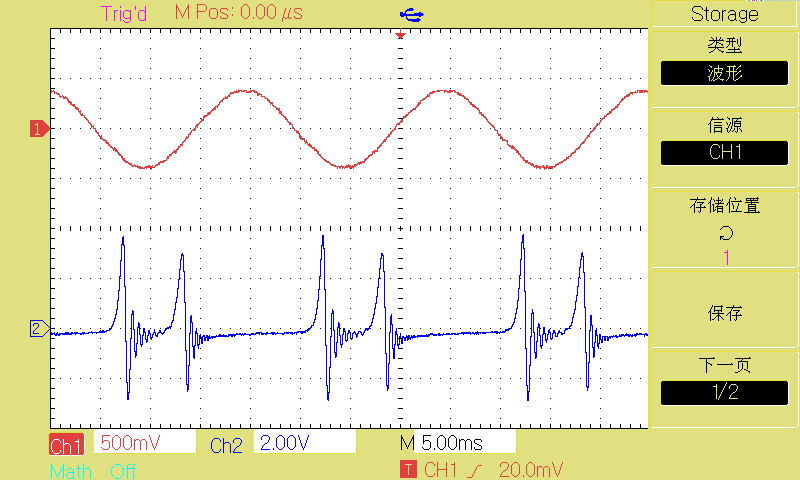
\includegraphics[width=60mm]{./dat/pics/prc/continuous/1unequal.png}\label{subfig:1unequal}}\hspace{1cm}
		\subfloat[调节信号等宽]{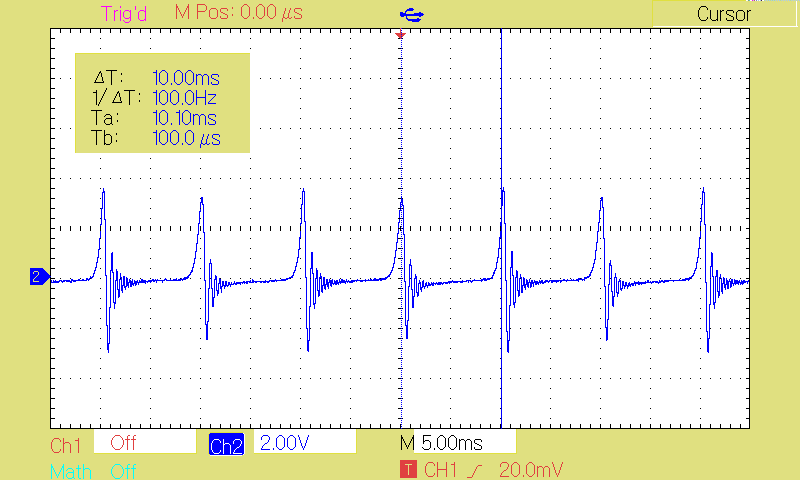
\includegraphics[width=60mm]{./dat/pics/prc/continuous/2equal.png}\label{subfig:2equal}}
		\caption{5%CuSO\textsubscript{4}水溶液样品共振信号}\label{fig:Continuous1}
	\end{figure}
	根据\cref{eq:kkk},测量图中每组信号的中包络线相对无共振时电平的高度下降到其最大值(共振峰)的约$1-\dfrac{1}{\mathrm{e}}$处位置与对应共振峰的时间差,即为样品的表观横向弛豫时间$T_2^*$。又据\cref{eq:deltab},测量相关参数,即可计算磁场的不均匀度$\Delta B^*$。测量结果见\cref{tab:Continuous}。由此得出的平均值为
	\begin{equation}
		\dfrac{\Delta B^*}{B_0}=4.79\times 10^{-5}.
	\end{equation}
	\par 再按同样的方法分别测量 1%、0.5%、0.05%的 CuSO\textsubscript{4}水溶液和纯水的共振信号的形状(如\cref{fig:Continuous2})并计算样品的表观横向弛豫时间$T_2^*$和磁场的不均匀度相对值$\Delta B^*/B_0$,结果亦见\cref{tab:Continuous}。另由\cref{fig:Continuous2}可见,硫酸铜浓度越低,共振信号之前的信号就越多,再纯水中则与共振信号之后的尾波几乎等长。这可能是因为浓度较低时,此前的衰减更多地是由不同磁场强度区域的磁化强度进动不同造成的,一旦重新汇合便又能形成峰值,即色散信号$u$。下文的实验结果将表明,低浓度溶液样品的实际的弛豫时间其实已经超过这里的共振峰间距(50ms),证实此处的推测。\\
	\begin{figure}
		\centering
		\subfloat[5%CuSO\textsubscript{4}水溶液共振信号]%
		{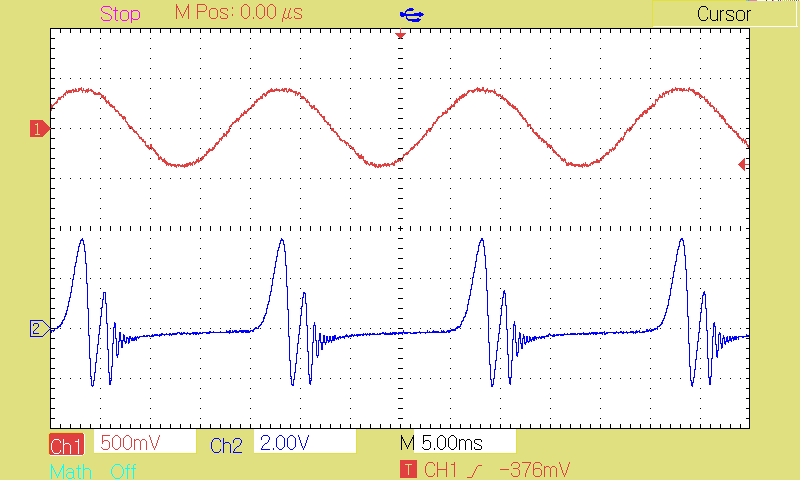
\includegraphics[width=50mm]{./dat/pics/prc/continuous/3CuSO4.1pc.png}\label{subfig:3CuSO4.1pc}}%
		\hspace{0.5cm}
		\subfloat[0.5%CuSO\textsubscript{4}水溶液共振信号]%
		{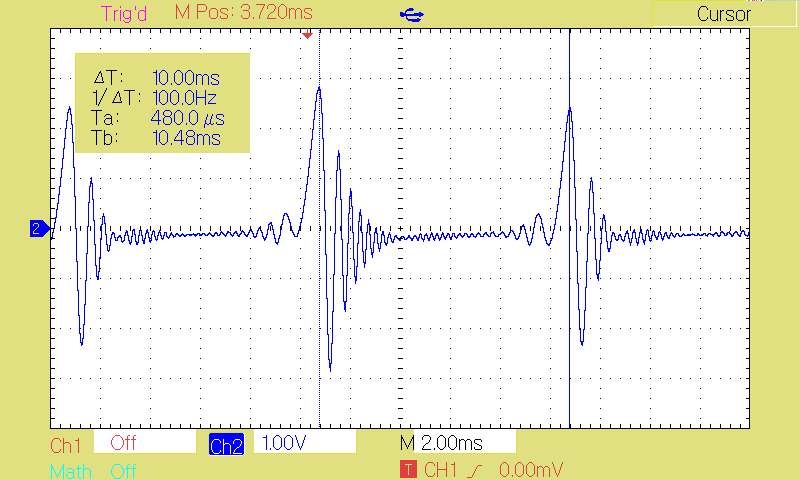
\includegraphics[width=50mm]{./dat/pics/prc/continuous/4CuSO4.0.5pc.png}\label{subfig:4CuSO4.0.5pc}}%
		\hspace{0.5cm}
		\subfloat[纯水共振信号]{\includegraphics[width=50mm]%
		{./dat/pics/prc/continuous/5Water.png}\label{subfig:5Water}}
		\caption{不同浓度CuSO\textsubscript{4}水溶液及纯水样品共振信号}\label{fig:Continuous2}
	\end{figure}
	\begin{table}[htbp!]
	\centering
	\caption{连续核磁共振实验结果}\label{tab:Continuous}	\begin{tabular}{c||c|c|c|c|c}
		\hline\hline
		CuSO$_4$浓度 & 5\% & 1\% & 0.5\% & 0.05\% & 0\\		\hline\hline
		共振频率$f_0$/Hz & 21.512 & 21.509 & 21.507 & 21.504 & 21.503\\		\hline
		共振峰高$y_0$/V & 4.08 & 3.06 & 2.50 & 1.73 & 0.43\\		\hline
		第一尾波峰位置$x_1$/ms & 0.7800 & 0.7900 & 0.8100 & 0.8400 & 0.8700\\		\hline
		第一尾波峰高$y_1$/V & 1.98 & 1.77 & 1.56 & 1.11 & 0.224\\		\hline
		第二尾波峰位置$x_2$/ms & 1.260 & 1.270 & 1.300 & 1.330 & 1.360\\		\hline
		第二尾波峰高$y_2$/V & 0.960 & 1.02 & 0.900 & 0.650 & 0.126\\		\hline
		第三尾波峰位置$x_3$/ms & 1.660 & 1.660 & 1.690 & 1.720 & 1.740\\		\hline
		第三尾波峰高$y_3$/V & 0.480 & 0.600 & 0.540 & 0.390 & 0.076\\		\hline
		第四尾波峰位置$x_4$/ms & 2.000 & 1.990 & 2.030 & 2.050 & 2.070\\		\hline
		第四尾波峰高$y_4$/V & 0.240 & 0.370 & 0.350 & 0.270 & 0.080\\		\hline
		尾波消失位置$x_0$/ms & 3.550 & 3.330 & 3.320 & 3.570 & 3.840\\		\hline
		表观横向弛豫时间$T^{*}_2$/ms & 0.9900 & 1.130 & 1.310 & 1.350 & 1.290\\		\hline
		$\Delta B^*/B_0$测量值 & 6.44$\times 10^{-5}$ & 4.52$\times 10^{-5}$ & 4.10$\times 10^{-5}$ & 4.16$\times 10^{-5}$ & 4.73$\times 10^{-5}$\\		\hline\hline
	\end{tabular}
\end{table} % tab:Continuous
	\par 比较不同浓度下信号的最大值和$T_2^*$(如\cref{fig:ContinuousCompare}),可见硫酸铜溶液共振峰的强度随着浓度的增大而增大,且都强于纯水的共振强度,这是由于	水中添加的顺磁离子(这里是Cu\textsuperscript{2+})含有未成对电子,%在外磁场作用下发生了({\color{red}???})
	顺磁离子的未成对电子可以增大每个氢核周围的局部磁场,促进它们的磁矩相位解相干,缩短其横向弛豫时间$T_2$;而实验结果中$T_2^*$随浓度变化的变化不大,这说明\cref{eq:deltab}中外磁场不均匀度对表观横向弛豫时间的贡献占了主要部分,外磁场不均匀度过大,无法由此估计实际的横向弛豫时间。
	\begin{figure}[htbp]
		\centering
		\subfloat[不同浓度下信号的最大值]{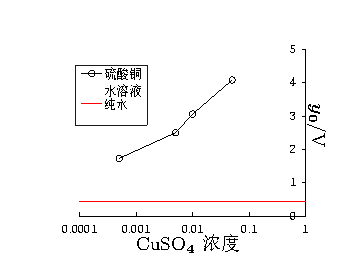
\includegraphics[width=80mm]{./dat/xlsxs/InitialSpikeHeight.pdf}\label{subfig:InitialSpikeHeight}}\hspace{1cm}
		\subfloat[不同浓度下信号的$T_2^*$值]{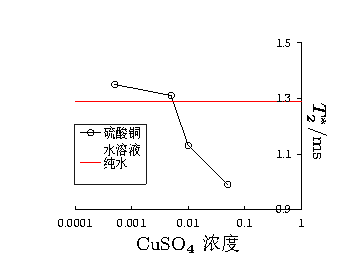
\includegraphics[width=80mm]{./dat/xlsxs/ApparentTransverseRelaxationTime.pdf}\label{subfig:ApparentTransverseRelaxationTime}}
		\caption{5%CuSO\textsubscript{4}水溶液样品共振信号}\label{fig:ContinuousCompare}
	\end{figure}

% subsection 连续核磁共振实验 (end)
\subsection{脉冲核磁共振实验} % (fold)
	\label{sub:脉冲核磁共振实验}
	\par 按\cref{subfig:app1}连接仪器后,先将0.05\%CuSO\textsubscript{4} 样品放入样品池,关好盖板。打开PNMR脉冲核磁采集软件,点击\framebox{连续采集}按钮发射射频信号,频率设为20MHz。先将时脉冲间隔设为0.20ms,第一脉冲宽度设为10-20ms,第二脉冲宽度30-60ms,再仔细调节磁铁调场电源,小范围改变磁场,使得软件显示的共振信号(调节合适也可以观察到自旋回波信号)最强。这时调节主机面板上磁铁匀场电源使磁场均匀度最佳,即信号尾波最多、自旋回波最强。
	\subsubsection{横向弛豫时间测量} % (fold)
		\label{ssub:横向弛豫时间测量}
		\par 调节第一脉冲宽度使其作用时间满足90$^{\circ}$脉冲条件(第一FID信号最大),并调节第二脉冲宽度至第一脉冲宽度的两倍左右(因为仪器本身特性,并不完全是两倍关系)作为180$^{\circ}$脉冲,然后反复细调匀场电源、调场电源、第一脉冲宽度和第二脉冲宽度至自旋回波信号最大。取不少于6个间隔,测量不同脉冲间隔情况下回波信号的大小,进行指数拟合得到横向弛豫时间(如图);再指数拟合第一脉冲后的共振信号,得到表观横向弛豫时间(如\cref{fig:PulseAT,fig:PulseT})。测量结果见\cref{tab:Pulse}。
		\begin{figure}
			\centering
			\subfloat[0.05\%CuSO\textsubscript{9}(aq)]%
			{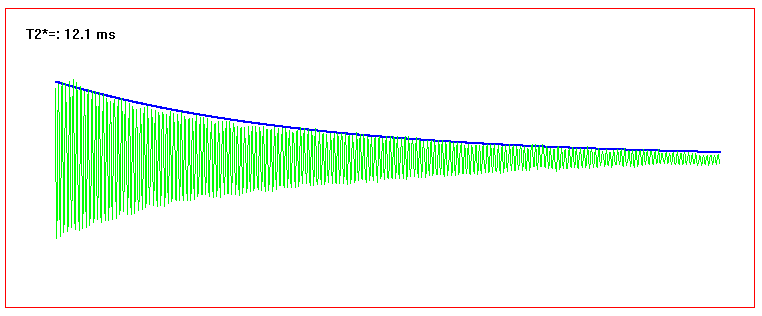
\includegraphics[width=50mm]{./dat/pics/prc/pulse/Apparent01.png}\label{subfig:at01}}%
			\hspace{0.5cm}
			\subfloat[0.1\%CuSO\textsubscript{4}(aq)]%
			{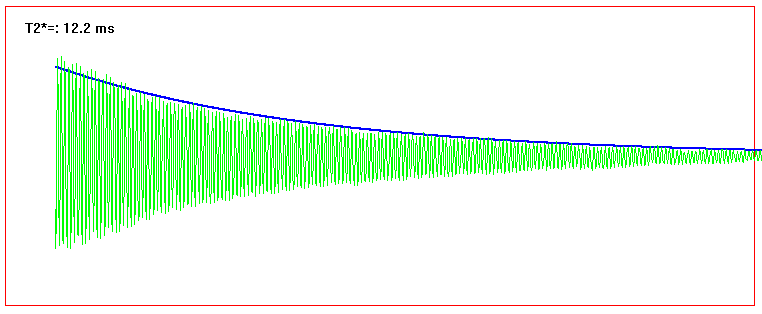
\includegraphics[width=50mm]{./dat/pics/prc/pulse/Apparent02.png}\label{subfig:at02}}%
			\hspace{0.5cm}
			\subfloat[0.3\%CuSO\textsubscript{5}(aq)]{\includegraphics[width=50mm]%
			{./dat/pics/prc/pulse/Apparent03.png}\label{subfig:at03}}\\
			\subfloat[0.5\%CuSO\textsubscript{6}(aq)]%
			{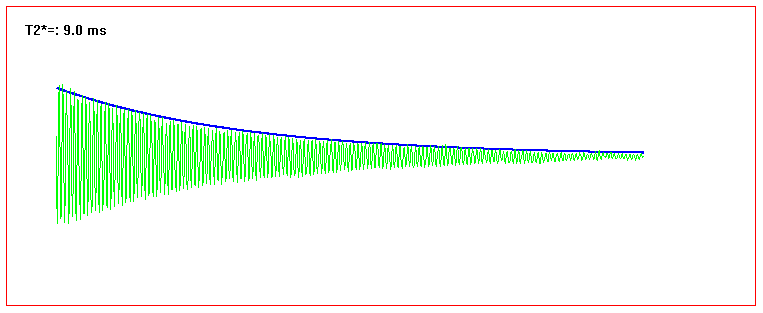
\includegraphics[width=50mm]{./dat/pics/prc/pulse/Apparent04.png}\label{subfig:at04}}%
			\hspace{0.5cm}
			\subfloat[1\%CuSO\textsubscript{7}(aq)]%
			{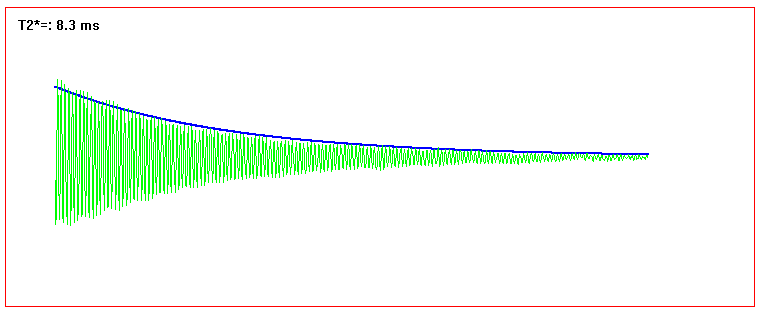
\includegraphics[width=50mm]{./dat/pics/prc/pulse/Apparent05.png}\label{subfig:at05}}%
			\hspace{0.5cm}
			\subfloat[纯水]{\includegraphics[width=50mm]%
			{./dat/pics/prc/pulse/Apparentwater.png}\label{subfig:atwater}}
			\caption{不同浓度CuSO\textsubscript{4}水溶液及纯水样品共振信号拟合表观横向弛豫时间}\label{fig:PulseAT}
		\end{figure}
		\begin{figure}
			\centering
			\subfloat[0.05\%CuSO\textsubscript{9}(aq)]%
			{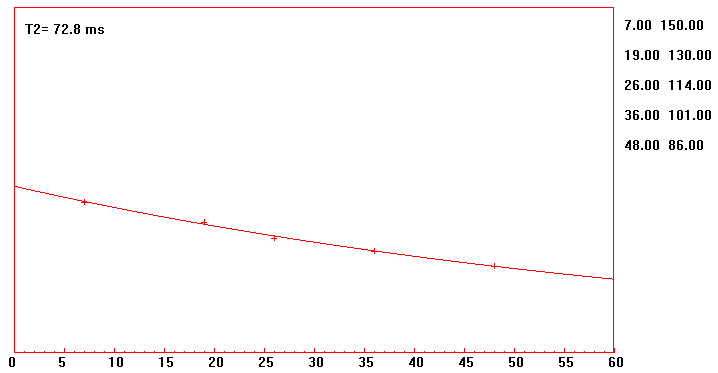
\includegraphics[width=50mm]{./dat/pics/prc/pulse/Transverse01.png}\label{subfig:t01}}%
			\hspace{0.5cm}
			\subfloat[0.1\%CuSO\textsubscript{4}(aq)]%
			{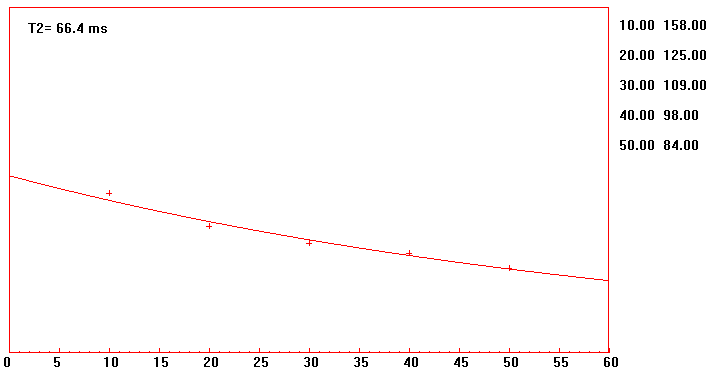
\includegraphics[width=50mm]{./dat/pics/prc/pulse/Transverse02.png}\label{subfig:t02}}%
			\hspace{0.5cm}
			\subfloat[0.3\%CuSO\textsubscript{5}(aq)]{\includegraphics[width=50mm]%
			{./dat/pics/prc/pulse/Transverse03.png}\label{subfig:t03}}\\
			\subfloat[0.5\%CuSO\textsubscript{6}(aq)]%
			{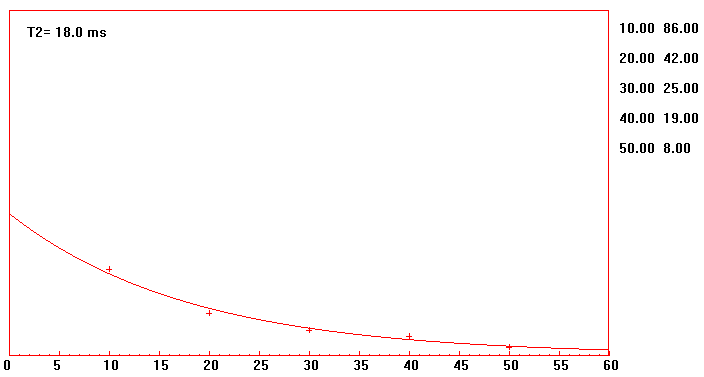
\includegraphics[width=50mm]{./dat/pics/prc/pulse/Transverse04.png}\label{subfig:t04}}%
			\hspace{0.5cm}
			\subfloat[1\%CuSO\textsubscript{7}(aq)]%
			{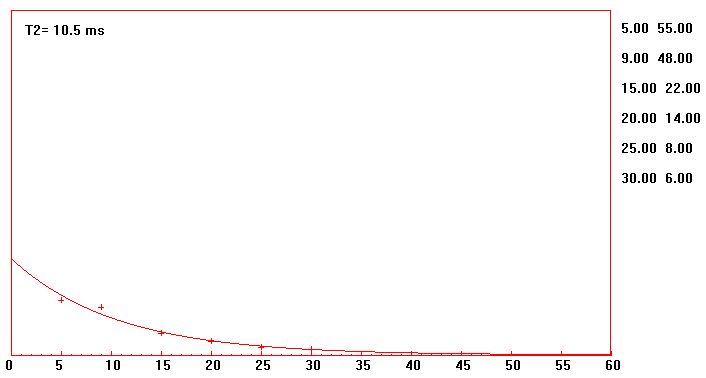
\includegraphics[width=50mm]{./dat/pics/prc/pulse/Transverse05.png}\label{subfig:t05}}%
			\hspace{0.5cm}
			\subfloat[纯水]{\includegraphics[width=50mm]%
			{./dat/pics/prc/pulse/Transversewater.png}\label{subfig:twater}}
			\caption{不同浓度CuSO\textsubscript{4}水溶液及纯水样品回波信号拟合横向弛豫时间}\label{fig:PulseT}
		\end{figure}
		\begin{table}[htbp!]
	\centering
	\caption{脉冲核磁共振实验结果}\label{tab:Pulse}	\begin{tabular}{c||c|c|c}
		\hline\hline
		$T_2$/ms & $T_2^*$/ms & $t_{\rm p,1}$/ms & 磁铁调场电源显示/V\\		\hline\hline
		66.4  & 12.2  & 0.30  & 2.55 \\		\hline
		39.4  & 9.3  & 0.26  & 2.54 \\		\hline
		18.0  & 9.0  & 0.26  & 2.54 \\		\hline
		10.5  & 8.3  & 0.26  & 2.54 \\		\hline
		 & 2.8  & 0.26  & 2.54 \\		\hline
		669.5  & 12.5  & 0.36  & 2.54 \\		\hline
		72.8  & 12.1  & 0.36  & 2.54 \\		\hline\hline
	\end{tabular}
\end{table}
	\FloatBarrier
	\begin{wrapfigure}[]{l}[0pt]{8cm}
	    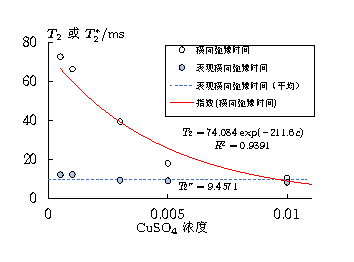
\includegraphics[width=80mm]{./dat/xlsxs/TransverseRelaxationTimeAndApparentTransverseRelaxationTime.pdf}\caption{横向弛豫时间和表观横向弛豫时间随样品中硫酸铜浓度的变化}\label{fig:t2t2starc}
	\end{wrapfigure}
	\FloatBarrier
		\cref{tab:Pulse}中数横向弛豫时间和表观横向弛豫时间随样品中硫酸铜浓度的变化关系如\cref{fig:t2t2starc}所示。由图可见,随着样品浓度的增大,表观横向弛豫时间基本不变,而实际横向弛豫时间大致按指数衰减。这说明水中添加的顺磁离子(这里是Cu\textsuperscript{2+})含有未成对电子,%在外磁场作用下发生了({\color{red}???})
		增大了每个氢核周围的局部磁场,促进它们的磁矩相位解相干,缩短其横向弛豫时间$T_2$;而$T_2^*$的测量中外磁场不均匀度对表观横向弛豫时间的贡献占了主要部分,外磁场不均匀度过大,随浓度变化的变化就很小。
	% subsubsection 横向弛豫时间测量 (end)
	\subsubsection{化学位移测量} % (fold)
		\label{ssub:化学位移测量}
		\par 分别放入甘油和二甲苯样品,调节匀场电源、调场电源使自旋回波信号最大,然后分别测量两种样品的相对化学位移。由\cref{fig:Continuous2CS}所示的实验结果可见,0.5%CuSO\textsubscript{4}水溶液的共振信号只有一个主要峰值,即只有一种氢核;而甘油和二甲苯的共振信号中则分别有1个(图中的三个极大值相距很近且起伏不大,没有超过噪声的幅度)和2个共振峰,说明其中分别有一种和两种氢核表现出核磁共振:甘油(CH$_2$OH-CHOH-CH$_2$OH)只有碳原子上的氢一种(羟基中的氢一般不表现),而二甲苯(CH$_3$C$_6$H$_6$CH$_3$)有甲基上的氢和苯环上的氢两种。
	\begin{figure}
		\centering
		\subfloat[0.5%CuSO\textsubscript{4}水溶液共振信号]%
		{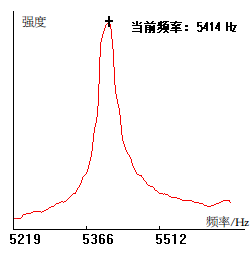
\includegraphics[width=40mm]{./dat/pics/prc/pulse/cuso4.png}\label{subfig:4CuSO4.0.5pcCS}}%
		\hspace{0.5cm}
		\subfloat[二甲苯样品共振信号]%
		{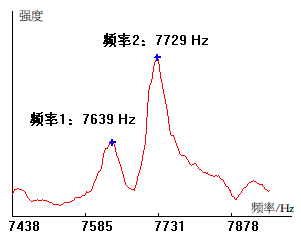
\includegraphics[width=55mm]{./dat/pics/prc/pulse/c6h6ch32.png}\label{subfig:3CuSO4.1pcCS}}%
		\hspace{0.5cm}
		\subfloat[甘油样品共振信号]{\includegraphics[width=55mm]%
		{./dat/pics/prc/pulse/hoch2ch2ohch2oh.png}\label{subfig:5WaterCS}}
		\caption{不同浓度CuSO\textsubscript{4}水溶液及纯水样品共振信号}\label{fig:Continuous2CS}
	\end{figure}
		\par \cref{fig:Continuous2CS}中的各个峰值测量结果见\cref{tab:cs}。根据\cref{eq:omega0,eq:delta}可以化得
		\begin{equation}
			\delta = \dfrac{\omega_{\rm S}-\omega_{\rm R}}{\omega_{\rm S}}\times 10^{6}.
		\end{equation}
		由此算出甘油和二甲苯中各极大值对硫酸铜溶液中氢原子的相对化学位移如\cref{tab:cs}。而二甲苯两个峰之间的相对化学位移则为
		\begin{equation}
			\delta = \dfrac{\Delta \omega}{\omega}\times 10^{6}=1.171\times 10^{4}\,\mathrm{ppm}.
		\end{equation}
		\begin{table}[htbp!]
	\centering
	\caption{化学位移测量结果\label{tab:cs}}\begin{tabular}{c||c|c|c|c}
		\hline\hline
		样品 & 共振峰频率/Hz & 相对化学位移$\delta$/ppm & $t_{\mathrm{p,1}}$/ms & 磁铁调场电源显示/V\\		\hline\hline
		0.5%CuSO\textsubscript{4}水溶液(参考) & 5414 & 0 & 0.20 & 2.60\\		\hline
		甘油 & 7370, 7390, 7407 & 0.2654, 0.2674, 0.2691 & 0.20 & 2.60\\		\hline
		二甲苯 & 7639, 7729 & 0.2912, 0.2995 & 0.20 & 2.60\\		\hline\hline
	\end{tabular}
\end{table}
	% subsubsection 化学位移测量 (end)
% subsection 脉冲核磁共振实验 (end)
%脉冲核磁共振实验
	%横向弛豫时间与样品浓度的关系。
%结合连续核磁共振和脉冲核磁共振的实验结果,以及讲义中的公式44,解释表观横向弛豫时间和横向弛豫时间与CuSO\(_4\)水溶液浓度变化关系差异较大的原因。
%结合在脉冲核磁实验中获得的横向弛豫时间与浓度的关系,分析在连续核磁共振实验中,不同浓度CuSO\(_4\)水溶液样品共振信号形状不同的原因。提示:比较扫场周期和横向弛豫时间不的大小关系和
%分析为什么甘油的核磁共振信号没有化学位移而二甲苯却有?提示:两者的分子结构不同。
